\subsection{Maximale Leistung bei variabler Spannung}\label{subsec:LeistungSpannungsabfall}
In diesem Versuch wird die maximale Leistung bei einem Spannungsabfall untersucht. Da die asynchrone Maschine nicht für 3800 RPM ausgelegt ist, wird dieser Versuch bei einer konstanten Drehzahl von 3600 RPM gemessen. Die weiteren Parameter können der Tabelle \ref{tab:maxLeistung} entnommen werden.

\begin{table}[H]
	\centering
	\begin{tabular}{C{4cm} C{4cm} C{3cm}} 
		\multicolumn{3}{c}{\textbf{Versuchsbedingungen}} \\
		{Messgrösse}& {Bedingung} & {Wert}\\ \hline\hline 
		Spannung (DC)   & variiert &   80-90 V     \\
		Strom (DC)   & gemessen &   9.94-100 A     \\
		Leistung (AC)   & gemessen &   223-6866 W    \\
		Drehzahl   & konstant &   3600 RPM    \\
		Drehmoment-Sollwert   & konstant &   max.    \\
		Motor-Temperatur   & vernachlässigt &   -    \\
		Controller-Temperatur   & vernachlässigt &   -    \\
	\end{tabular}
	\caption{Versuchsbedingungen max. Leistung}\label{tab:maxLeistung}
\end{table}

Unter der Annahme, dass zwischen der maximalen Leistung und der Spannung ein quadratischer Zusammenhang besteht (Abbildung \ref{fig:maxLeistung}, rote Approximation), ist anzunehmen, dass die maximale Leistung bei 3600 RPM und Nennspannung (96V) bei 15kW liegt. Da die Leistung auf der AC-Seite gemessen wurde, wird wie bei den vorherigen Versuchen für die ASM ein Wirkungsgrad von 90\% angenommen.

\begin{figure}[H]
	\centering
	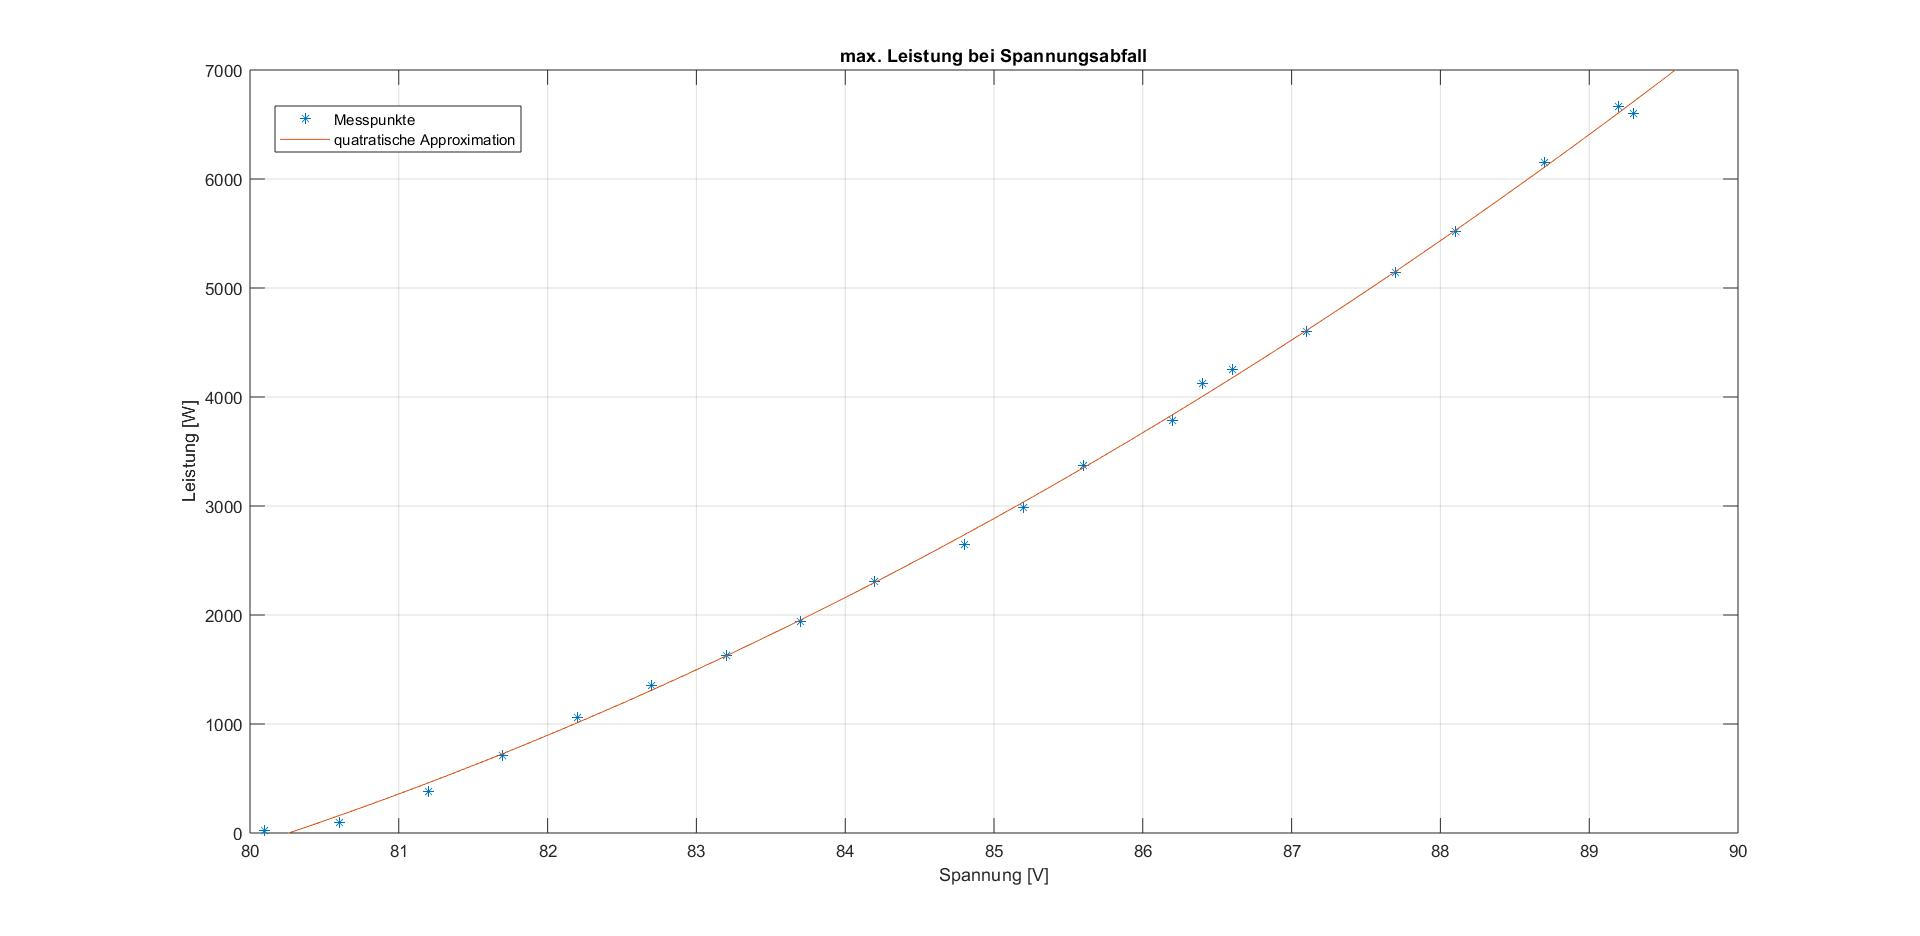
\includegraphics[width=0.9\linewidth]{maxLeistung.jpg}
	\caption{Maximale Leistung}\label{fig:maxLeistung}
\end{figure}

Es ist gut ersichtlich, dass die quadratische Approximation praktisch perfekt an die Messpunkte anliegt. Es kann daher mit gutem gewissen gesagt werden, dass die Leistung bei Spannungsabnahme quadratisch abnimmt. Dieser Zusammenhang gilt jedoch lediglich für Spannungen unterhalb der Motoren Nennspannung von 96V.